% !TEX root = ../main.tex

\chapter{预备知识}
本章将介绍本论文所涉及的关键技术背景：零知识证明、零知识简洁非交互式知识论证、PLONKish算术化方案、零知识虚拟机以及程序验证技术。零知识证明是一种允许证明者在不泄露任何额外信息的前提下向验证者证明计算正确性的密码学协议。零知识简洁非交互式知识论证通过多项式约束和双线性配对实现了简洁且非交互的证明生成与验证。PLONKish算术化方案提供了将任意计算转换为多项式约束系统的强大框架。零知识虚拟机在高层程序与底层约束系统之间引入抽象层，使得复杂程序的零知识证明生成更加高效。程序验证技术则通过将程序正确性问题归约为布尔可满足性问题，利用SAT求解器实现自动化验证，符号执行作为一种重要的程序分析方法，通过探索程序路径和生成路径约束来检测程序漏洞和验证可达性属性。

\section{零知识证明与算术电路}

\subsection{零知识证明}
零知识证明（Zero-Knowledge Proof, ZKP）是一种运行在证明者和验证者之间的密码学协议，允许证明者在不泄露任何额外信息的前提下，向验证者证明某个计算的正确性\cite{DBLP:journals/siamcomp/GoldwasserMR89}。零知识证明的核心原理在于：验证者除了获知计算结果的有效性之外，无法获取任何其他信息~\cite{cryptoeprint:2024/457}。设$x$表示待证明的陈述，$w$表示见证（即私有输入），$L$表示有效陈述的语言集合。在零知识证明协议中，证明者$P$生成一个证明$\pi$，用以证明$(x,w) \in R_{L}$，其中$R_{L}$是定义语言$L$的关系。该证明需满足以下三个核心性质\cite{DBLP:conf/crypto/GoldreichMW86}：

\begin{description}
    \item[完备性] 完备性描述了协议的正确性。对于所有满足$(x,w) \in R_{L}$的实例，诚实的证明者$P$能够使诚实的验证者$V$以概率1相信该计算是正确的。换言之，如果证明者确实掌握了有效的见证，那么验证者必定会接受该证明。
    
    \item[可靠性] 可靠性确保恶意证明者无法欺骗验证者接受错误的陈述。对于所有$x \notin L$的情况以及任意恶意证明者$P^{*}$，$P^{*}$使验证者$V$接受的概率在安全参数$\lambda$下是可忽略的，即$\Pr[V(x,\pi) = 1] \leq \text{negl}(\lambda)$。这一性质保证了即使证明者试图作弊，验证者也几乎不可能被欺骗。
    
    \item[零知识性] 零知识性意味着验证者除了获知陈述的正确性之外，无法获取任何其他信息。形式化地，存在一个多项式时间模拟器$S$，对于所有$(x,w) \in R_{L}$，验证者的视图与$S(x)$在计算上不可区分。这确保了验证者无法通过证明过程推断出关于见证$w$的任何信息。
\end{description}

这三个性质共同确保了零知识证明能够提供安全且隐私保护的计算验证方法，在不暴露敏感信息的前提下完成正确性验证。

如图 \ref{fig:1} 所示，该图展示了零知识证明（Zero-Knowledge Proof）的基本交互模型。证明者P拥有某个声明X的证据或知识，需要向验证者V证明该声明的真实性。与传统证明方式不同，零知识证明允许证明者生成一个简洁的证据（proof），并将其发送给验证者，验证者通过验证该证据来判断声明X的有效性，最终做出接受或拒绝的决策。零知识证明的核心特性在于：证明者能够使验证者确信声明为真，但除了"声明为真"这一事实外，验证者无法从证据中获取任何额外信息~\cite{JinruiSHA2024185812}，从而实现了知识的零泄露。这种非交互式的证明系统相比传统交互式证明具有更高的效率，证据可以被多次验证而无需证明者重复参与，使其特别适用于区块链等去中心化场景。

\begin{figure}[htbp]
    \centering
    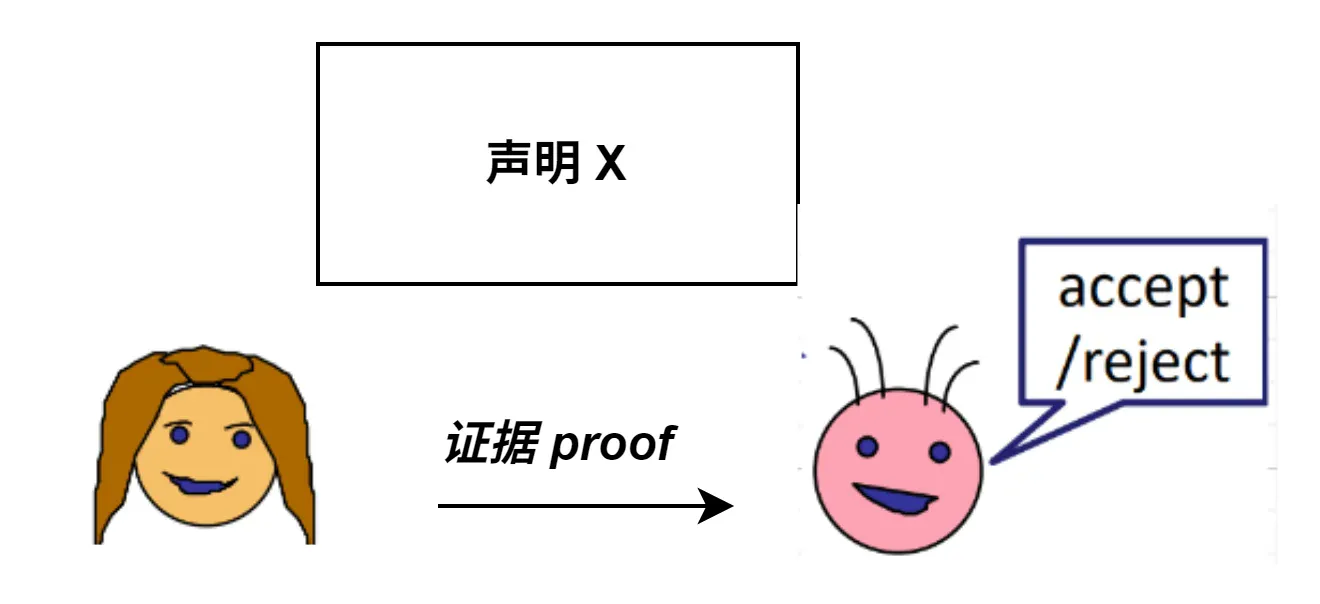
\includegraphics[width=0.6\linewidth]{figures/1.png}
    \bicaption{零知识证明的证明模型}{Proof Model for Zero-Knowledge Proofs} % 双语标题
    \label{fig:1}
\end{figure}

根据交互方式的不同，零知识证明可分为交互式和非交互式两类\cite{DBLP:conf/stoc/BlumFM88}。在交互式零知识证明中，证明者和验证者需要进行多轮通信才能完成证明过程。证明者$P$首先提供一个承诺（Commitment），等待验证者$V$发起挑战（Challenge），然后根据挑战中的随机值进行回应（Response）。如果证明者确实能够证明命题的正确性，那么他将能够顺利通过每轮挑战；否则，他只能以一定的概率通过每轮挑战。验证者通过多轮挑战来评估证明的有效性，当认为证明正确的概率达到足够高时，才认可该证明。

\subsection{简洁非交互式零知识证明}

简洁非交互式零知识证明（Zero-Knowledge Succinct Non-Interactive Argument of Knowledge, zkSNARK）在零知识证明的基础上引入了简洁性和非交互性两大核心特征，使其特别适合于在保护隐私的同时验证复杂计算\cite{Groth10}。在zkSNARK中，证明规模保持恒定，不随计算复杂度的增加而增长，且验证过程无需证明者与验证者之间的交互。

zkSNARK的核心思想是将计算转换为有限域$\mathbb{F}$上的多项式约束系统\cite{ben-zksnark}，其中$\mathbb{F}$具有素数阶$p$。设$\mathcal{C}$为待证明的计算，$w$为其见证（私有输入）。计算被编码为一组多项式方程：
$$\mathcal{C}(x,w) = 0 \iff \{p_{i}(x,w) = 0\}_{i=1}^{m}$$
其中$p_{i}: \mathbb{F}^{n} \rightarrow \mathbb{F}$是次数至多为$d$的多项式。

这种编码方式利用了多项式的一个基本性质：两个次数为$d$的不同多项式最多在$d$个点上取值相同~\cite{Bayer2013ZeroKnowledgeAF}。因此，对于随机选取的$r \in \mathbb{F}$，如果$p(r) = q(r)$，则$p = q$的概率至少为$1 - d/|\mathbb{F}|$。这一性质使得验证者可以通过在单个随机点检验多项式相等性来高效完成验证，而无需检查整个多项式。\cite{10.1007/978-3-031-51479-1_18}

\begin{figure}
    \centering
    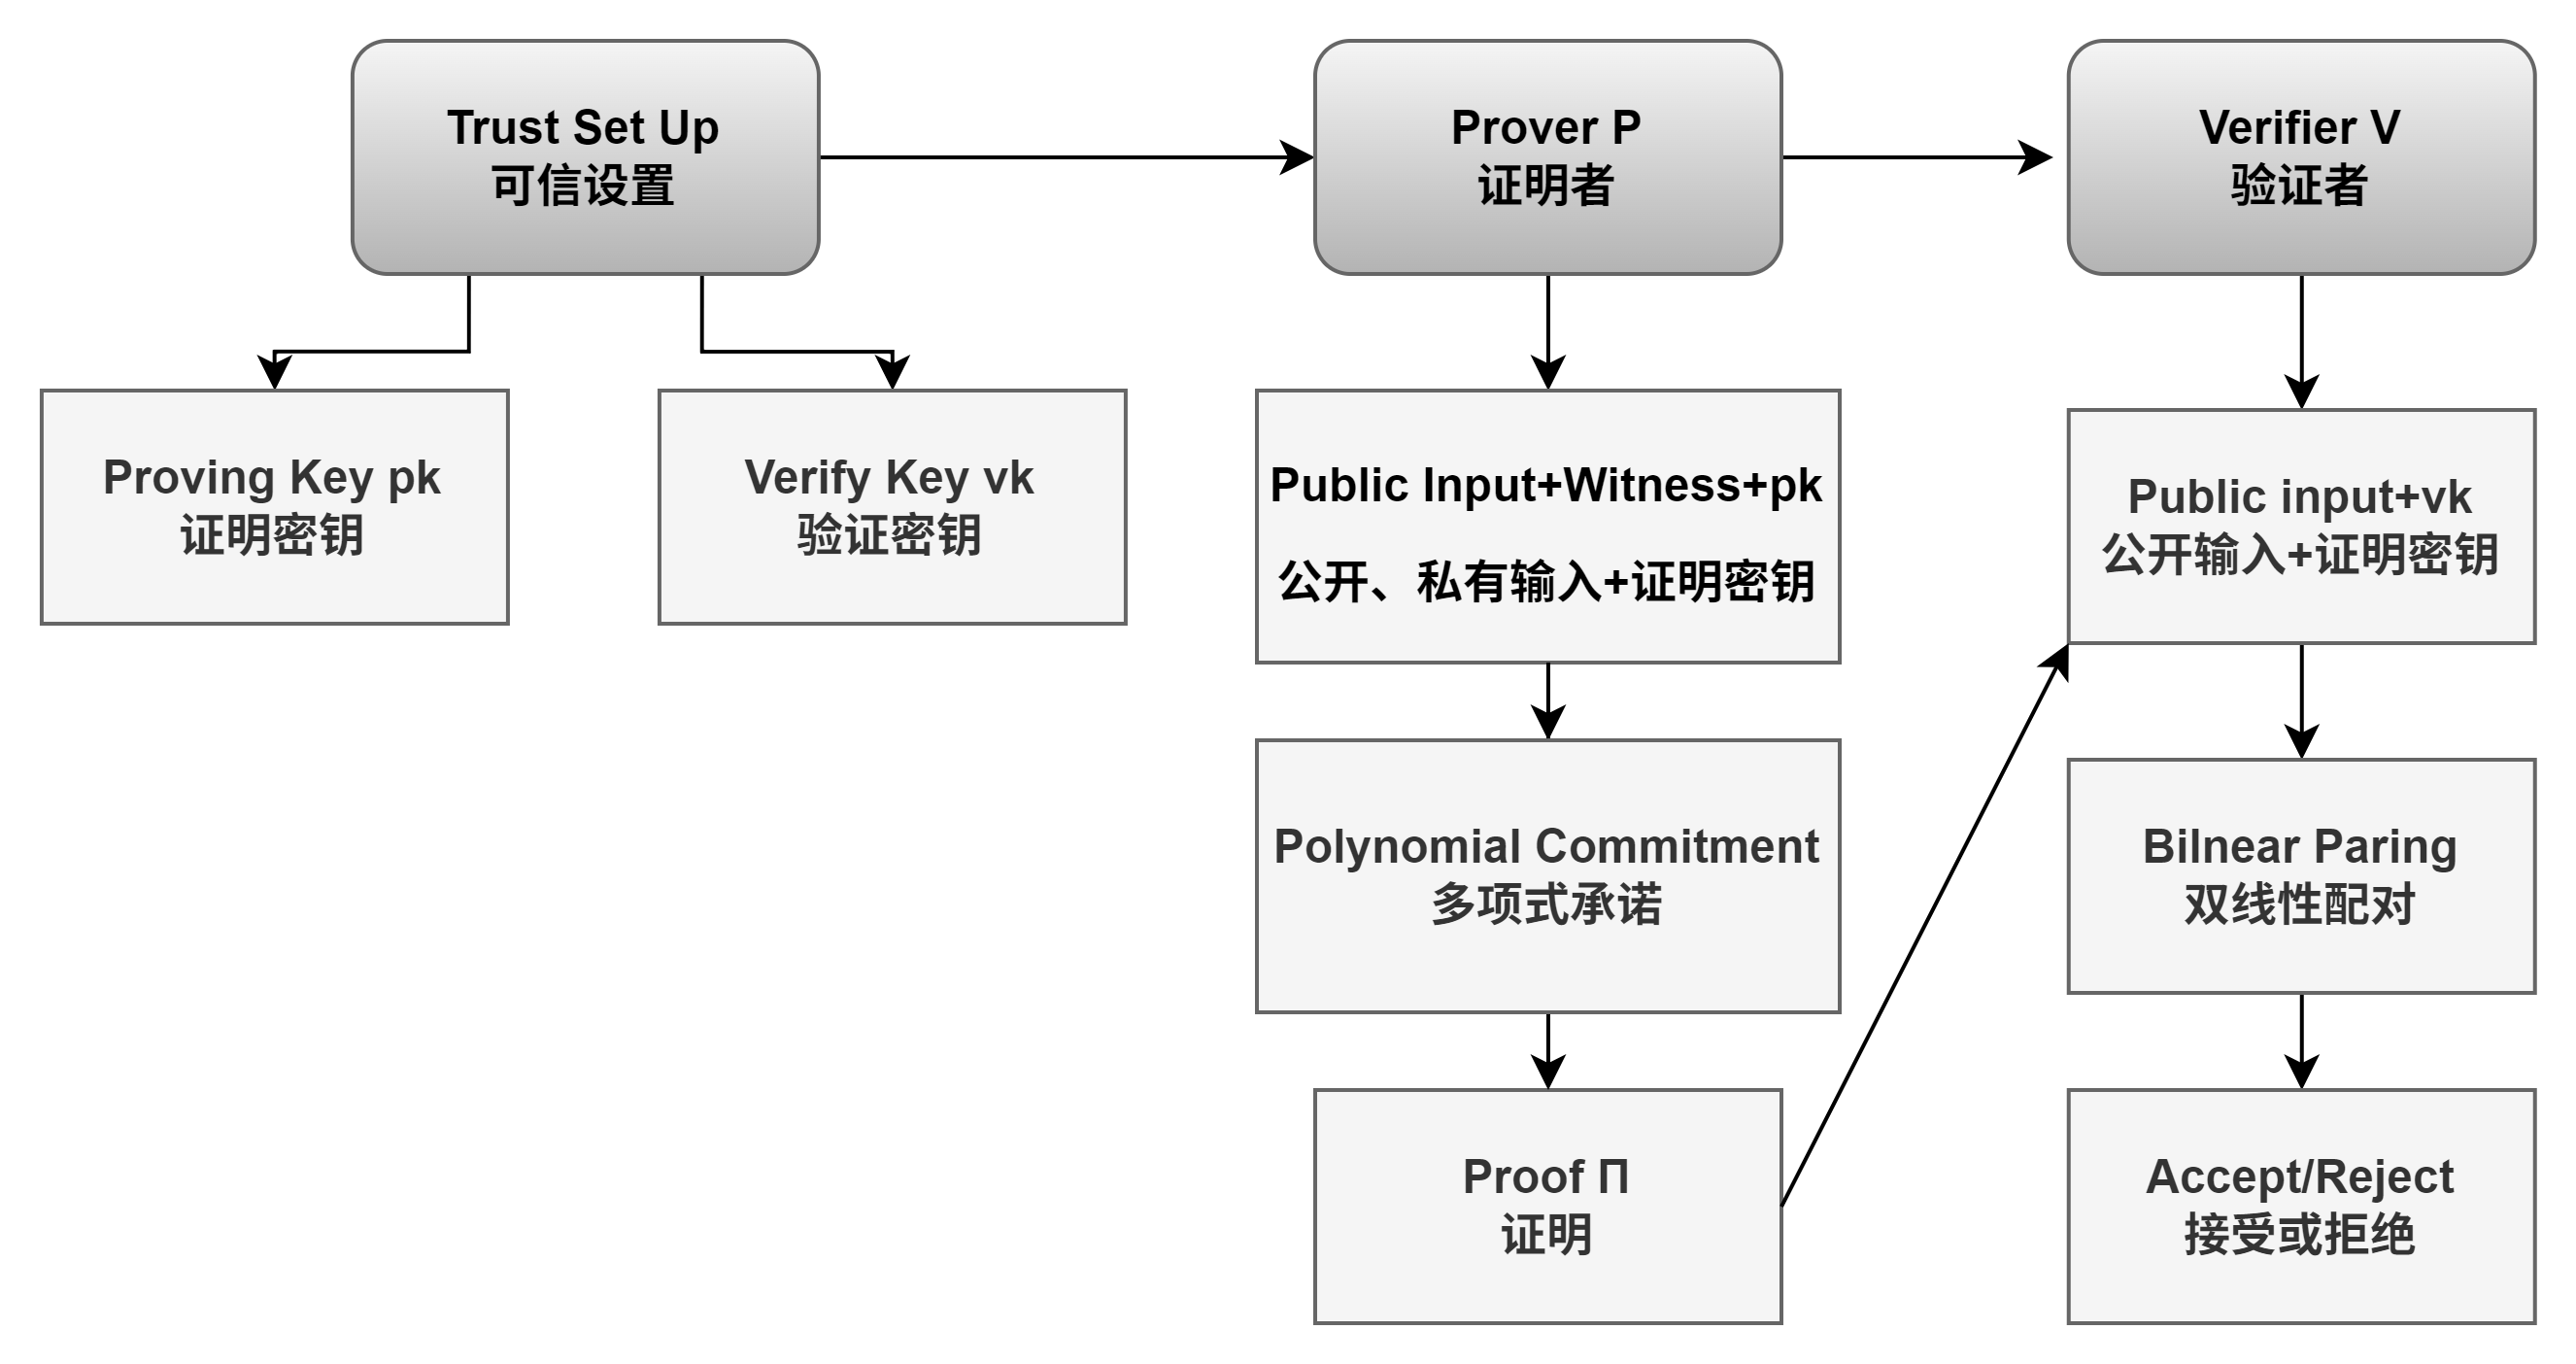
\includegraphics[width=0.9\linewidth]{figures/2.png}
    \bicaption{简洁非交互式零知识证明执行流程}{Execution flow of succinct non-interactive zero-knowledge proof}
    \label{fig:zksnark-flow}
\end{figure}

为了在实现验证的同时保持零知识性，zkSNARK采用了双线性配对技术\cite{DBLP:conf/asiacrypt/Groth10}。设$\mathbb{G}_{1}$、$\mathbb{G}_{2}$、$\mathbb{G}_{T}$为素数阶$p$的循环群，生成元分别为$g_{1}$、$g_{2}$。双线性配对$e: \mathbb{G}_{1} \times \mathbb{G}_{2} \rightarrow \mathbb{G}_{T}$满足以下性质：对于所有$a, b \in \mathbb{Z}_{p}$，有$e(g_{1}^{a}, g_{2}^{b}) = e(g_{1}, g_{2})^{ab}$。这一性质允许在加密值上进行算术运算——验证者可以检验$p(r) = 0$是否成立，而无需获知见证$w$或多项式的具体取值。

如图\ref{fig:zksnark-flow}所示，简洁非交互式零知识证明（zkSNARK）的执行流程包含三个核心阶段。在可信设置（Trusted Setup）阶段，系统生成证明密钥$pk$和验证密钥$vk$，这两个密钥将分别用于后续的证明生成和验证过程。在证明阶段，证明者$\mathcal{P}$将公开输入、私有见证与证明密钥$pk$作为输入，通过多项式承诺机制生成简洁的证明$\pi$。在验证阶段，验证者$\mathcal{V}$仅需公开输入、证明$\pi$与验证密钥$vk$，通过双线性配对运算即可高效完成验证，输出接受或拒绝的结果。整个过程中，证明者与验证者之间无需交互，且证明规模保持恒定，不随计算复杂度增长。

zkSNARK的简洁性源于多项式承诺机制，复杂的计算被归约为常数规模的多项式求值\cite{ye2025yoimiyascalableframeworkoptimal}。零知识性则通过双线性配对实现，使得验证可以在加密值上进行。这种技术组合使得zkSNARK成为生成复杂计算证明的理想选择，能够在隐藏敏感计算细节的同时完成正确性验证。

\subsection{普朗克算术系统}

为了构建zkSNARK证明，计算必须首先被转换为多项式约束系统，这一过程称为算术化（Arithmetization）。PLONKish提供了一种强大的算术化框架，在高层计算与zkSNARK所需的多项式方程之间架起了桥梁\cite{DBLP:journals/iacr/GabizonWC19}。

设$\mathbb{F}$为有限域，$\mathcal{C}$为具有公共输入$x$和私有见证$w$的计算。PLONKish通过构造矩阵$M \in \mathbb{F}^{k \times n}$将$\mathcal{C}$转换为约束系统，其中每一行代表一个计算步骤。其核心思想在于：$\mathcal{C}(x,w)$有效当且仅当矩阵$M$上的某些多项式关系成立。

具体而言，PLONKish通过三类多项式约束对计算进行编码：

\begin{description}
    \item[门约束（Gate Constraints）] 门约束将计算操作转换为多项式方程。对于每种操作类型，多项式$p_{g}: \mathbb{F}^{m} \rightarrow \mathbb{F}$编码其语义：
    $$p_{g}(M_{i,c_{1}}, M_{i,c_{2}}, ..., M_{i+r,c_{3}}) = 0, \quad \forall i \in [k]$$
    这使得zkSNARK可以通过证明这些多项式求值为零来证明计算的正确性。门约束的灵活性在于可以定义自定义门（Custom Gates），从而高效地表达特定的计算模式。\cite{10.1007/978-3-031-68403-6_11}
    
    \item[复制约束（Copy Constraints）] 复制约束在电路中建立多项式相等关系：
    $$M_{i_{1},j_{1}} - M_{i_{2},j_{2}} = 0$$
    这些约束实现了值在电路不同位置之间的传播，同时保持了高效zkSNARK证明生成所需的多项式结构。复制约束通过置换论证（Permutation Argument）高效实现，确保同一变量在不同位置的取值一致。
    
    \item[查找约束（Lookup Constraints）] 查找约束将某些操作归约为多项式包含性检查：
    $$(f_{1}(M_{i}), ..., f_{m}(M_{i})) \in T \subseteq \mathbb{F}^{m}$$
    通过预计算查找表$T$，范围检查等操作可以简化为简单的多项式求值，而非复杂的代数表达式。这一机制显著减少了约束数量，提升了证明效率。\cite{cryptoeprint:2023/1518}

    \item[置换约束（Shuffle Constraints）] 置乱约束要求矩阵$M$中的两列$a$与$b$作为元素集合满足集合相等性：两列必须包含完全相同的元素且重数一致，而与元素顺序无关。形式化表示为：
    $$\{a_{i}\}_{i \in [k]} =_{\text{multiset}} \{b_{i}\}_{i \in [k]}$$
    置换约束常用于证明某列是另一列的重排列，该约束通过多重集合论证（Multiset Argument）高效实现，验证者无需知晓具体的置换映射即可确认集合相等性。
\end{description}

如图\ref{fig:plonk-accumulator}所示，基于PLONKish算术化的累乘器约束通过执行轨迹矩阵实现。矩阵包含四个核心列：私有见证列$X_{a,i}$、$X_{b,i}$、$X_{c,i}$分别存储每行的输入与输出值（证明者私有数据），公开选择器列$Q_{p,i}$用于控制该行是否启用乘法门。系统对各列施加了以下约束：\textbf{(1) 门约束（Gate Constraints）}：当$Q_{p,i} = 1$时，要求$c_i = a_i \cdot b_i \cdot c_{i-1}$成立，即当前输出等于两个输入与前一行输出的乘积；当$Q_{p,i} = 0$时，该行仅用于初始化。\textbf{(2) 复制约束（Copy Constraints）}：通过置换论证（Permutation Argument）确保$X_{c,i}$在第$i$行的输出值正确传递到第$i+1$行作为$c_{i-1}$使用，保证累乘的连续性。\textbf{(3) 边界约束}：第$i=0$行的$c_0$作为公开输入，最终行的$c_k$作为公开输出，验证者可验证累乘结果。该设计通过门约束实现单步计算逻辑，复制约束保证跨行数据一致性，无需查找表即可高效证明累乘运算的正确性。

\begin{figure}
    \centering
    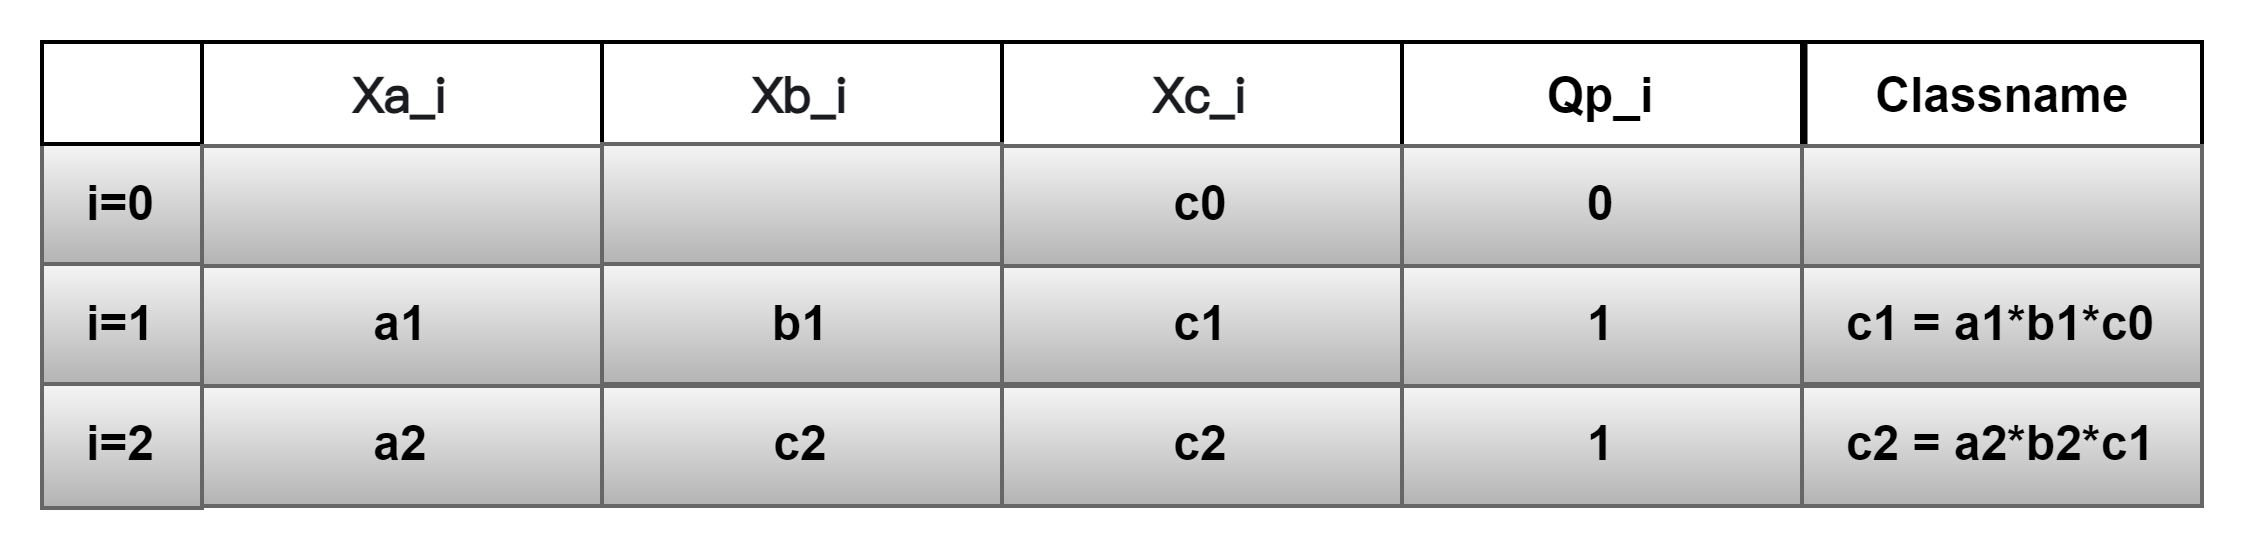
\includegraphics[width=0.85\linewidth]{figures/3.png}
    \bicaption{基于PLONKish算术化的累乘器约束}{Product accumulator constraints based on PLONKish arithmetization}
    \label{fig:plonk-accumulator}
\end{figure}

PLONKish的优雅之处在于将任意计算转换为zkSNARK可高效证明的统一多项式形式。证明者通过展示所有多项式约束求值为零来证明其掌握有效见证$w$，而zkSNARK的简洁性确保证明规模保持恒定，不随计算规模增长\cite{cryptoeprint:2019/953}。这种算术化方法通过自定义门和查找表提供了编码多样计算模式的灵活性，使其成为当前最广泛采用的zkSNARK算术化方案之一。

相比于传统的R1CS约束系统，PLONKish具有更强的表达能力和更高的证明效率。R1CS\cite{10.1007/978-3-031-15979-4_5}要求每个约束具有固定的二次形式$\langle a, s \rangle \cdot \langle b, s \rangle = \langle c, s \rangle$，而PLONKish允许定义任意次数的自定义门，并通过查找表支持非算术操作。这种灵活性使得PLONKish特别适合于表达复杂的程序验证任务，为后续章节介绍的零知识虚拟机提供了底层支撑。

\subsection{零知识虚拟机}\label{zkvm}

虽然PLONKish算术化为编码计算提供了强大的框架，但随着程序复杂性的增长，直接为复杂程序构造算术电路变得越来越具有挑战性。zkVM通过在高级程序和低级约束系统之间引入抽象层来解决这一可扩展性挑战。\cite{wang2025surveyinteractiveverifiablecomputing}

zkVM是一种专门为生成程序执行的zkSNARK证明而设计的虚拟机架构~\cite{10.1007/978-3-031-58751-1_1}。设$\mathcal{P}$为程序，$I$为其输入，$S = (s_0, s_1, \ldots, s_T)$为执行轨迹，其中每个$s_i$表示步骤$i$时的机器状态\cite{2025arXiv250817518G}。zkVM通过证明状态转换的有效性来证明$\mathcal{P}(I)$产生输出$O$：
$$s_{i+1} = \delta(s_i, \text{inst}_i), \quad \forall i \in [0, T-1]$$
其中$\delta$是状态转换函数，$\text{inst}_i$是步骤$i$处执行的指令。

zkVM的核心思想是将复杂计算分解为简单、统一操作的序列\cite{10.1007/978-3-031-91134-7_6}。zkVM不是为每个程序创建自定义电路，而是定义一个固定的指令集架构（ISA），其中每条指令都有相应的约束模板。执行轨迹随后被编码为：
$$\mathcal{C}_{\text{zkVM}} = \bigwedge_{i=0}^{T-1} \mathcal{C}_{\text{inst}_i}(s_i, s_{i+1})$$
其中$\mathcal{C}_{\text{inst}}$表示每种指令类型的约束集合。

\begin{figure}
    \centering
    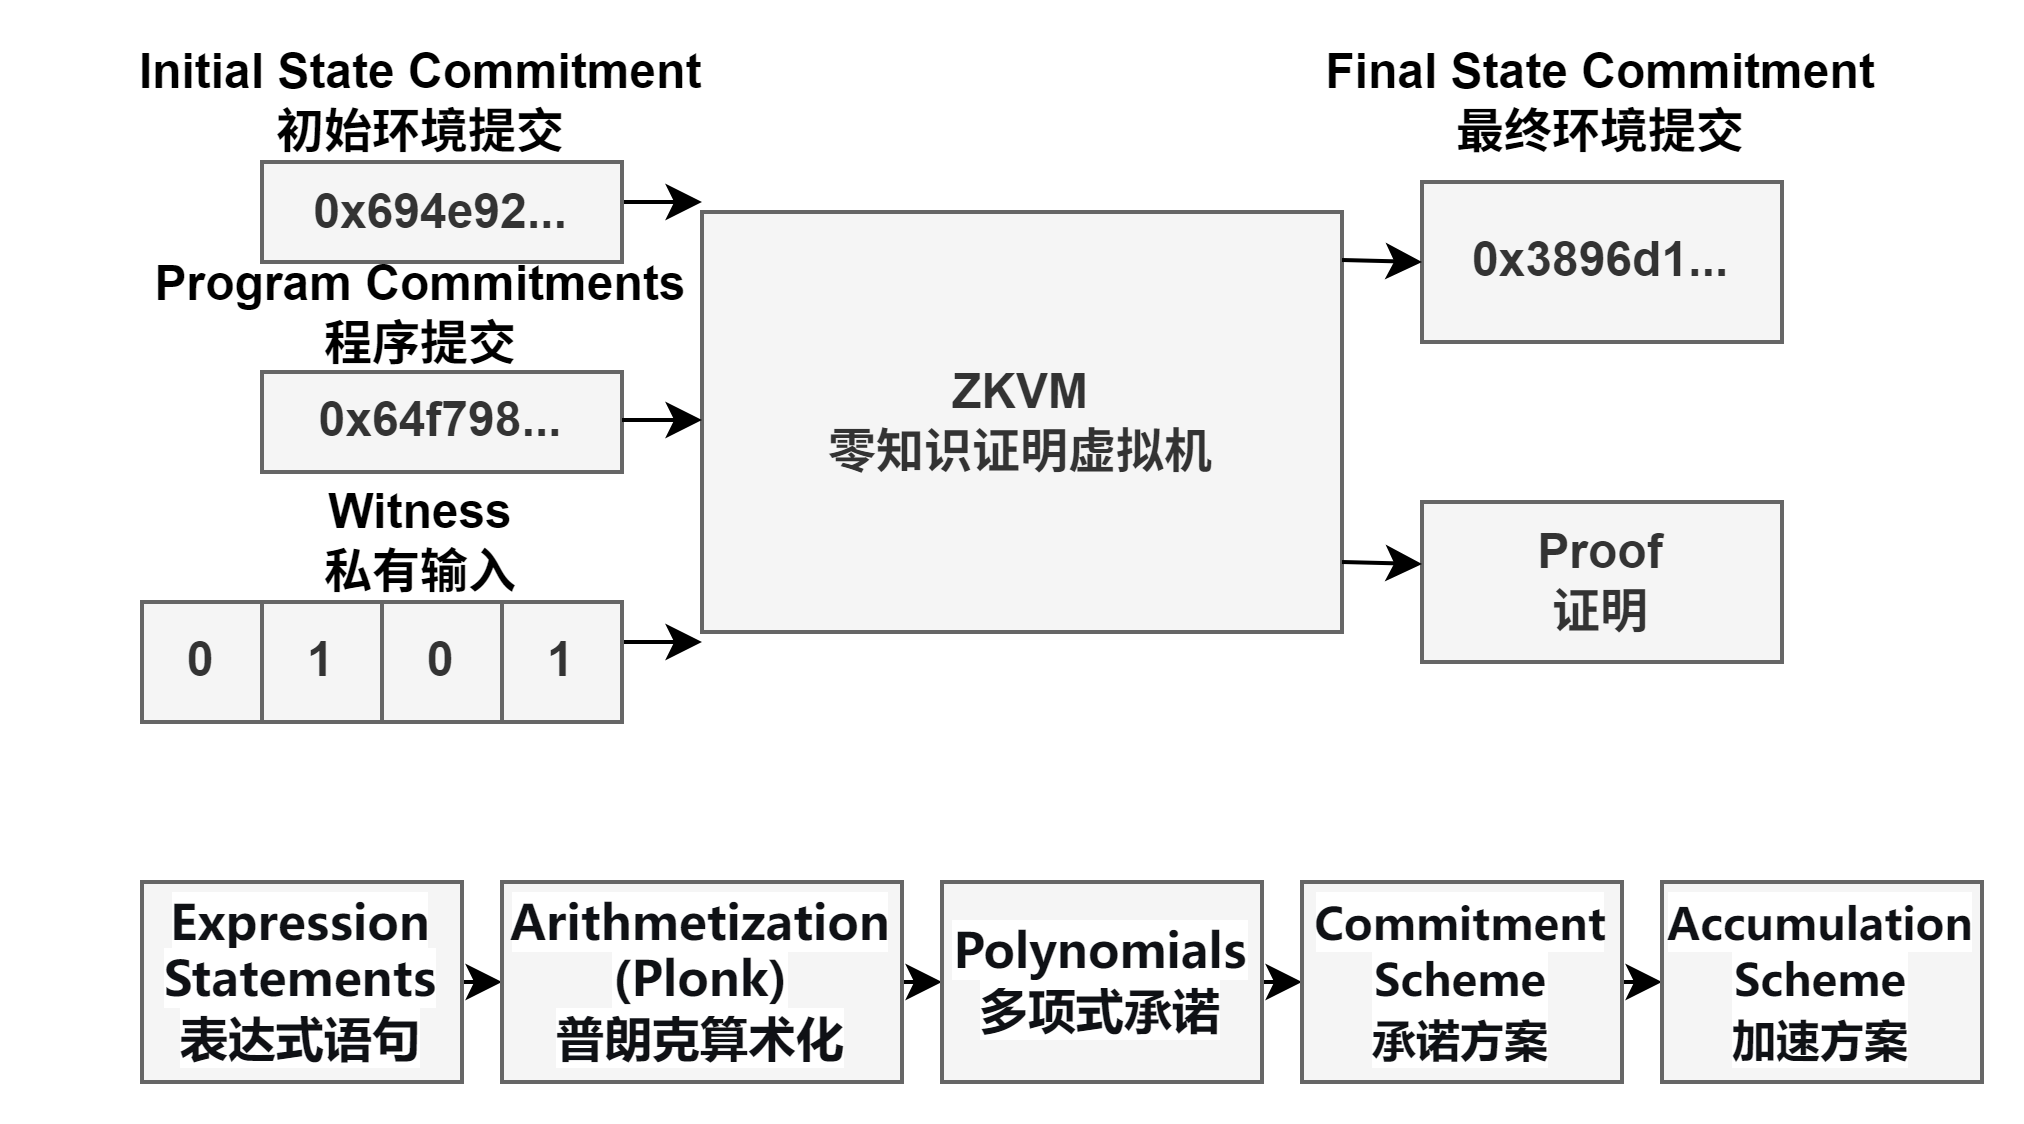
\includegraphics[width=0.85\linewidth]{figures/4.png}
    \bicaption{ZKVM零知识证明虚拟机架构}{ZKVM (Zero-Knowledge Virtual Machine) Architecture}
    \label{fig:zkvm-architecture}
\end{figure}

如图\ref{fig:zkvm-architecture}所示，ZKVM零知识证明虚拟机通过五层架构实现从高级程序到零知识证明的完整转换流程。系统以待证明程序的字节码（如0x694e92...、0x64f798...等）及输入数据（如0101序列）作为私有见证数据，输出最终证明（Proof）供验证者验证。架构的五个核心层次为：\textbf{(1) 表达式语句层（Expression Statements）}：将程序执行转换为一系列表达式语句，描述计算的语义逻辑。\textbf{(2) 算术化层（Arithmetization/Plonk）}：采用PLONKish算术化方案，将表达式语句转化为约束系统，包括门约束、复制约束和查找约束，形成执行轨迹矩阵。\textbf{(3) 多项式层（Polynomials）}：将约束系统编码为多项式形式，利用多项式承诺的代数性质实现高效证明。\textbf{(4) 承诺方案层（Commitment Scheme）}：对多项式进行密码学承诺，常用方案包括KZG承诺或FRI承诺，确保证明的简洁性与安全性。\textbf{(5) 累加方案层（Accumulation Scheme）}：通过证明累加技术实现递归证明或批量验证，进一步压缩证明规模。整个架构通过层层转换，将通用计算转化为可验证的零知识证明，实现了程序执行正确性的高效可验证性。

这种架构相比直接算术化提供了几个关键优势。首先，内存操作通过具有地址-值对$(a, v) \in \mathbb{F} \times \mathbb{F}$的全局内存模型统一处理。其次，控制流通过程序计数器$pc \in \mathbb{F}$管理，该计数器对指令执行进行排序。第三，模块化的指令约束使得证明组合和优化成为可能。\cite{cryptoeprint:2020/1069}

从程序到证明的转换遵循两阶段过程：程序$\mathcal{P}$首先被编译为zkVM字节码，然后zkVM执行生成使用zkSNARK证明的约束。这种关注点分离使得zkVM能够处理任意程序复杂性，同时保持高效的证明生成，因为电路大小仅取决于执行轨迹长度而非程序结构~\cite{cryptoeprint:2024/387}。

\section{程序验证}
\subsection{程序验证的布尔可满足性归约}

程序验证通过形式化方法证明软件满足其规约，确保正确性属性成立\cite{Lanzinger_2024}。设$P$表示程序，$\phi$表示规约属性，记号$P \models \phi$表示程序$P$满足属性$\phi$。在基于SAT的验证中，验证问题被归约为布尔可满足性问题。该归约构造公式$\psi$使得$\psi$可满足当且仅当$P$违反属性$\phi$，从而利用高度优化的SAT求解器实现自动化验证。常见的基于SAT的方法包括界限为$n$的有界模型检测（Bounded Model Checking）和路径集为$\Pi$的符号执行（Symbolic Execution）。

具体而言，程序$P$首先被转换为静态单赋值形式（Static Single Assignment, SSA）$P_{SSA}$以便进行SAT编码。对于界限为$n$的有界验证，设状态空间$\mathcal{S}$中的状态序列为$s_0, s_1, ..., s_n$，初始条件谓词为$I$，则验证条件$VC(P_{SSA}, \phi, n)$定义为：
$$VC(P_{SSA}, \phi, n) = I(s_0) \wedge \bigwedge_{i=0}^{n-1} \tau(s_i, s_{i+1}) \wedge \neg\phi(s_n)$$
其中，转移关系$\tau: \mathcal{S} \times \mathcal{S} \rightarrow \{0,1\}$刻画了程序的状态转移逻辑。程序在界限$n$内满足属性$\phi$当且仅当验证条件$VC(P_{SSA}, \phi, n)$不可满足。

SAT编码的核心在于编码函数$\mathcal{E}$，它将程序构造映射为布尔公式\cite{10.1007/978-3-540-24730-2_15}。对于$m$位变量$v$，位向量$b^v = \{b_0^v, b_1^v, ..., b_{m-1}^v\}$满足$b_i^v \in \{0,1\}$，其编码为$\mathcal{E}(v) = b^v$。对于算术运算$op$及其对应的布尔电路$C_{op}$，二元运算的编码为$\mathcal{E}(v_1\ op\ v_2) = C_{op}(b^{v_1}, b^{v_2})$。对于包含条件序列$\{c_1, c_2, ..., c_k\}$的执行路径$\pi$，路径编码为$\mathcal{E}(\pi) = \bigwedge_{i=1}^{k} \mathcal{E}(c_i)$，即所有路径条件的合取。

最终，SAT求解器判定编码公式$\psi = \mathcal{E}(VC(P_{SSA}, \phi, n))$的可满足性。若$\psi$可满足，则满足赋值提供了具体的反例，展示程序如何违反属性$\phi$；若$\psi$不可满足，则证明程序在界限$n$内满足该属性。这种反例驱动的验证方法在软件工程中广泛应用，特别是在安全关键系统的形式化验证中。

\begin{figure}
    \centering
    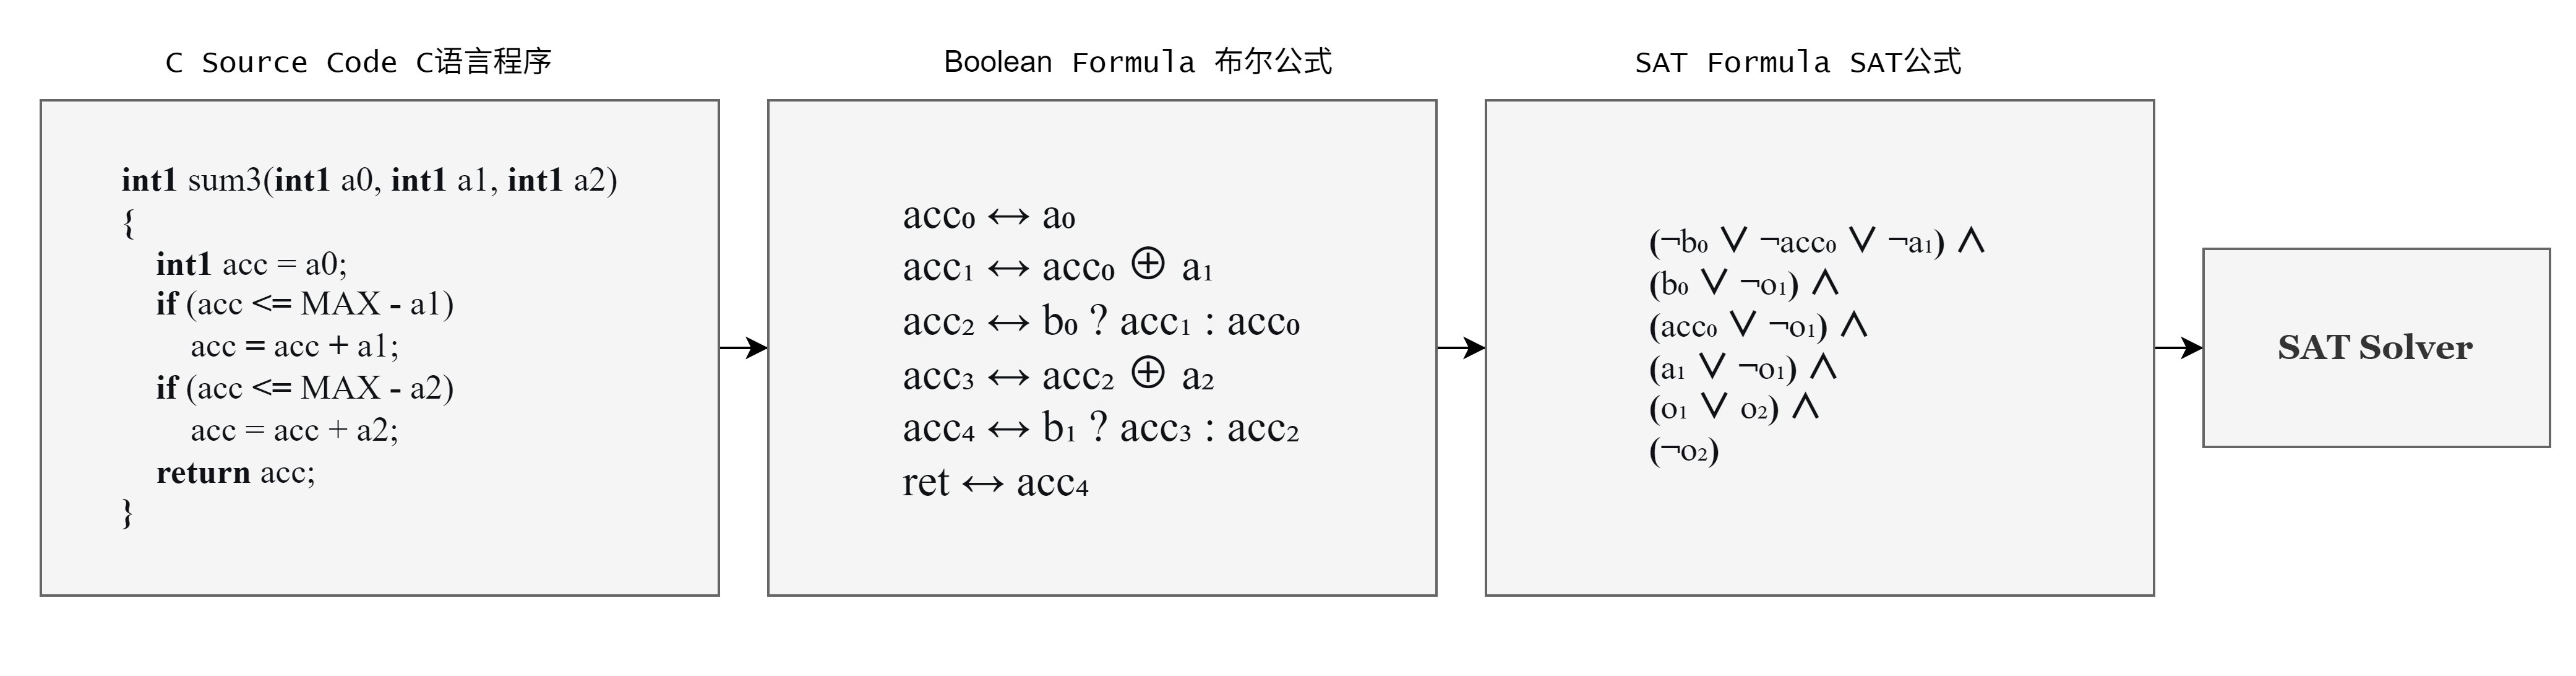
\includegraphics[width=0.85\linewidth]{figures/5.png}
    \bicaption{从C程序到SAT公式的编码流程}{Encoding pipeline from C program to SAT formula}
    \label{fig:sat-encoding}
\end{figure}

    如图\ref{fig:sat-encoding}所示，基于SAT的程序验证通过三阶段编码流程将C源代码转换为可由SAT求解器判定的布尔公式。以sum3函数为例，该函数接收三个整型参数a0、a1、a2，通过累加操作计算返回值，并在每次加法前检查是否超过上界MAX。编码流程的三个核心阶段为：\textbf{(1) 布尔公式生成（Boolean Formula）}：将C程序转换为逻辑表达式序列。累加器变量acc通过静态单赋值形式展开为$\text{acc}_0, \text{acc}_1, ..., \text{acc}_4$，初始化表示为$\text{acc}_0 \leftrightarrow a_0$；条件分支if语句转换为三元表达式，如$\text{acc}_2 \leftrightarrow b_0 \ ? \ \text{acc}_1 : \text{acc}_0$，其中$b_0$编码第一个条件判断；加法操作通过$\oplus$符号表示位级加法，如$\text{acc}_1 \leftrightarrow \text{acc}_0 \oplus a_1$；最终返回值关联为$\text{ret} \leftrightarrow \text{acc}_4$。\textbf{(2) SAT公式转换（SAT Formula）}：将布尔表达式转换为合取范式（CNF）。每个逻辑关系被分解为子句的合取，例如$\text{acc}_0$的定义转化为$(\neg b_0 \vee \neg \text{acc}_0 \vee \neg a_0)$等子句；条件表达式$b_0 \ ? \ \text{acc}_1 : \text{acc}_0$展开为多个蕴含关系，确保在$b_0$为真时选择$\text{acc}_1$，为假时选择$\text{acc}_0$；算术运算$\oplus$的位向量语义通过进位逻辑编码为布尔子句，如$(b_0 \vee \neg o_1) \wedge (a_1 \vee \neg o_1)$表示加法的部分逻辑；最终公式$(\neg o_2)$表示验证条件的否定，即寻找违反规约的反例。\textbf{(3) SAT求解器判定（SAT Solver）}：将CNF公式输入求解器进行可满足性判定。若公式可满足，求解器返回满足赋值（对应程序的反例执行路径）；若不可满足，则证明程序在给定界限内满足规约。该编码流程展示了程序验证如何通过逐层抽象降低，最终归约为纯布尔逻辑问题，使得高效的SAT求解算法得以应用于软件正确性证明。

    基于SAT的验证方法的优势在于其自动化程度高和反例生成能力强。现代SAT求解器（如Z3、MiniSat）利用冲突驱动子句学习（CDCL）等高效算法~\cite{serrano2024selfsatisfiedendtoendframeworksat}，能够处理包含数百万布尔变量的公式。然而，这种方法也存在局限性：有界验证仅能保证程序在有限步骤内的正确性，无法覆盖所有可能的执行路径；对于复杂程序，编码公式的规模可能随界限$n$指数增长，导致求解困难。尽管存在这些限制，SAT归约仍然是程序验证领域的重要技术。通过将程序语义转换为布尔逻辑，验证问题得以利用数十年来SAT求解器研究的成果。

\subsection{符号执行}
符号执行（Symbolic Execution）是一种程序分析技术，通过将程序输入抽象为符号值而非具体值来系统地探索程序的执行路径。与传统的具体执行（Concrete Execution）不同，符号执行维护一个符号状态$\sigma$（将变量映射到符号表达式）和一个路径约束$PC$（关于符号表达式的量词自由一阶公式）\cite{10.1007/978-3-540-24730-2_15}。在符号执行开始时，$\sigma$初始化为空映射，$PC$初始化为真值$\top$。当程序执行到条件分支语句时，符号执行引擎会"分叉"（fork）执行路径：对于条件表达式$e$，若$PC \wedge \sigma(e)$可满足，则沿"真"分支继续执行并更新路径约束为$PC' = PC \wedge \sigma(e)$；若$PC \wedge \neg\sigma(e)$可满足，则创建新的执行实例沿"假"分支执行并更新路径约束为$PC'' = PC \wedge \neg\sigma(e)$。这种系统化的路径探索使得符号执行能够自动生成触发特定程序行为的测试输入。

\begin{algorithm}[H]
    \SetAlgoLined
    \bicaption{符号执行算法}{Symbolic Execution Algorithm}
    \label{algo:symbolic-execution}
    \KwIn{程序$P$，输入空间$\mathcal{I}$，状态空间$\mathcal{S}$}
    \KwOut{测试输入集合$T \subseteq \mathcal{I}$}
    
    $\sigma_0 \leftarrow \emptyset$, $PC_0 \leftarrow \top$, $s_0 \leftarrow \text{entry}(P)$\;
    $W \leftarrow \{(s_0, \sigma_0, PC_0)\}$, $T \leftarrow \emptyset$\;
    
    \While{$W \neq \emptyset$}{
        $(s, \sigma, PC) \leftarrow \text{Select}(W)$\;
        $W \leftarrow W \setminus \{(s, \sigma, PC)\}$\;
        
        \uIf{$s$ 是赋值 $v := e$}{
            $W \leftarrow W \cup \{(\text{next}(s), \sigma[v \mapsto \sigma(e)], PC)\}$\;
        }
        \uElseIf{$s$ 是条件分支 $\texttt{if}\ e\ \texttt{then}\ s_1\ \texttt{else}\ s_2$}{
            \If{$\text{SAT}(PC \wedge \sigma(e))$}{
                $W \leftarrow W \cup \{(s_1, \sigma, PC \wedge \sigma(e))\}$\;
            }
            \If{$\text{SAT}(PC \wedge \neg\sigma(e))$}{
                $W \leftarrow W \cup \{(s_2, \sigma, PC \wedge \neg\sigma(e))\}$\;
            }
        }
        \uElseIf{$s$ 是终止语句}{
            $T \leftarrow T \cup \{\text{Solve}(PC)\}$\;
        }
    }
    \KwRet $T$\;
\end{algorithm}
    
    符号执行的核心执行流程可形式化描述为算法\ref{algo:symbolic-execution}。该算法维护一个工作列表$W$，存储待探索的符号执行状态，每个状态由程序位置$s$、符号状态$\sigma$和路径约束$PC$组成。算法初始化时，将程序入口点、空符号状态和真值路径约束作为初始状态加入工作列表。随后，算法迭代地从工作列表中选择状态进行探索：对于赋值语句，更新符号状态并继续执行后继语句；对于条件分支，调用SAT求解器判定两个分支的路径约束是否可满足，将可满足的分支状态加入工作列表，从而实现路径分叉；对于终止语句，调用约束求解器生成满足当前路径约束的具体测试输入。通过这种系统化的探索过程，符号执行能够覆盖程序的多条可行路径，并为每条路径生成相应的测试输入。

\begin{figure}
    \centering
    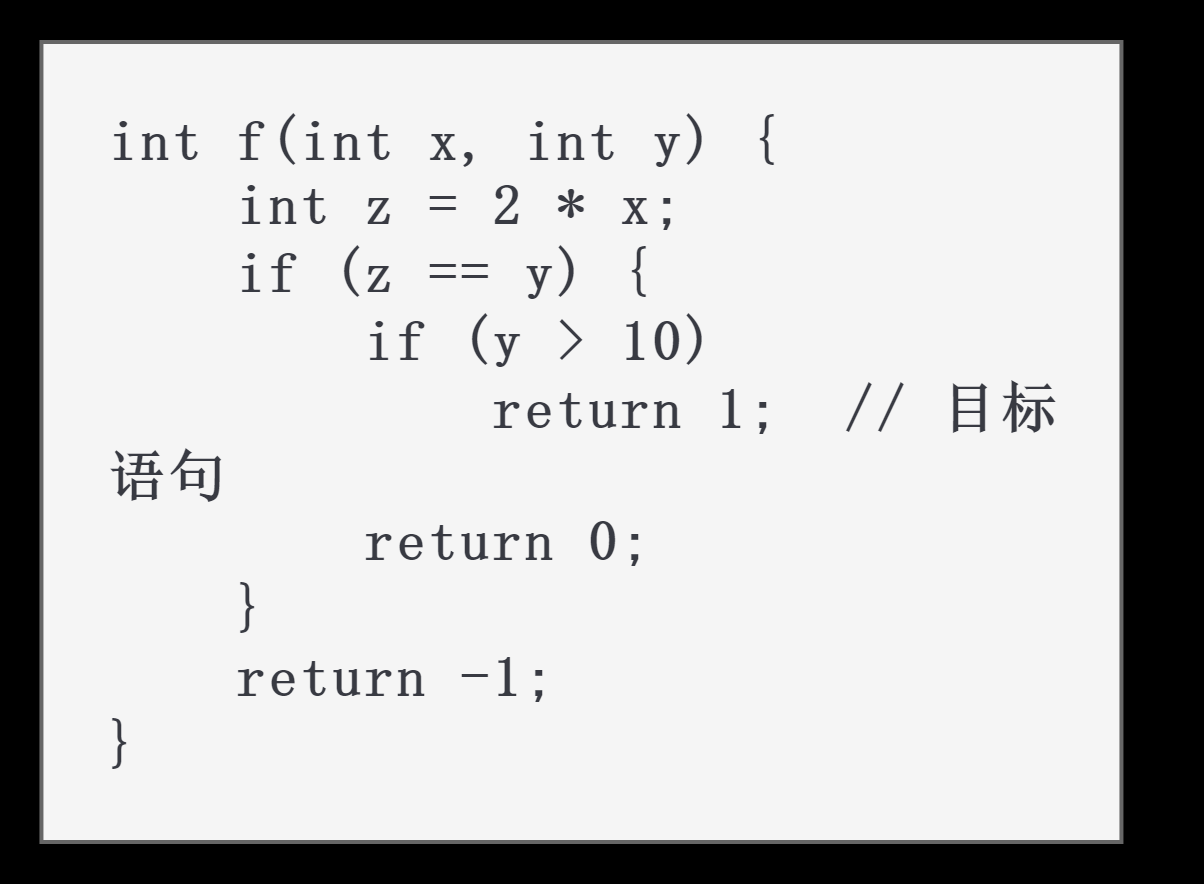
\includegraphics[width=0.6\linewidth]{figures/6.png}
    \bicaption{符号执行示例代码}{Example code for symbolic execution}
    \label{fig:symbolic-execution-example}
\end{figure}

    如图\ref{fig:symbolic-execution-example}所示，考虑一个简单的C函数作为符号执行的示例。在符号执行该函数时，输入参数$x$和$y$被赋予符号值$\lambda_x$和$\lambda_y$。执行第一行赋值语句后，符号状态更新为$\sigma(z) = 2 \cdot \lambda_x$。到达第一个条件分支时，引擎检查约束$2 \cdot \lambda_x = \lambda_y$的可满足性。由于该约束可满足，引擎沿真分支继续，路径约束更新为$PC_1 = (2 \cdot \lambda_x = \lambda_y)$；同时创建另一执行实例沿假分支探索，其路径约束为$PC_2 = (2 \cdot \lambda_x \neq \lambda_y)$。沿真分支继续执行到第二个条件时，需检查$PC_1 \wedge (\lambda_y > 10)$的可满足性。若可满足（例如$\lambda_x = 6, \lambda_y = 12$），则生成到达目标语句的测试输入；若不可满足，则该路径被剪枝。通过这种方式，符号执行系统地探索了函数的所有可行路径。

    在路径选择方面，由于完全探索所有路径不可行，符号执行工具采用启发式策略优先探索重要路径。常见策略包括：随机路径选择在每个分支随机选择方向，避免陷入局部；覆盖引导策略优先探索能够到达未覆盖代码的路径；深度优先或广度优先搜索分别侧重深入探索或广度覆盖。KLEE采用多策略交错执行，动态平衡不同目标。在约束处理方面，混合具体-符号执行（Concolic Execution）是重要技术：在符号执行的同时维护具体执行，当遇到难以求解的约束时用具体值替换符号值，确保执行能够继续。这种方法牺牲了完备性（可能错过某些路径），但显著提升了实用性。EXE和DART等工具采用执行生成测试（Execution-Generated Testing）范式，交替进行具体执行和符号分析，有效处理复杂程序。

\subsection{SAT/UNSAT的零知识证明系统}\label{sec:sat-proof}

    布尔可满足性问题（Boolean Satisfiability Problem, SAT）判定给定布尔公式是否存在使其求值为真的赋值。设$X = \{x_1, x_2, \ldots, x_m\}$为布尔变量集合，文字（literal）$l_{it}$为变量$x_j$（正文字）或其否定$\neg x_j$（负文字）。设$F^* = \{f^*_1, f^*_2, \ldots, f^*_n\}$为合取范式（CNF）布尔公式，其中每个$f^*_i$为子句（clause），由变量$X$上的文字析取组成。SAT求解器的输出为SAT（可满足）或UNSAT（不可满足），并需提供相应的证明以验证结果的正确性。
    
    \textbf{不可满足性证明（UNSAT Proof）:}
    对于不可满足公式$F^*$，归结证明（resolution proof）通过逐步推导最终得到空子句$\bot$来证明不存在满足赋值。设$D^* = \{d^*_1, d^*_2, \ldots, d^*_k\}$为导出子句序列，$T^* = \{t^*_1, t^*_2, \ldots, t^*_{2k}\}$为归结过程中使用的子句轨迹，$\text{pivot}_i$为第$i$步归结所使用的枢轴变量（pivot variable）。归结规则的核心在于：对于包含$\text{pivot}$和$\neg\text{pivot}$的两个父子句，通过消去枢轴变量生成归结式（resolvent）。为验证UNSAT结果，需满足以下关系：(1) 每个导出子句$d^*_i$或属于原始公式$F^*$，或通过归结规则从轨迹$T^* \subseteq \{F^* \cup D^*\}$中包含$\text{pivot}_i$和$\neg\text{pivot}_i$的两个父子句导出 (2) 导出子句$d^*_i$包含两个父子句的所有文字，但不包含$\text{pivot}_i$和$\neg\text{pivot}_i$，形式化表示为：若父子句为$C_1 = (\text{pivot}_i \vee l_1 \vee \cdots \vee l_p)$和$C_2 = (\neg\text{pivot}_i \vee l'_1 \vee \cdots \vee l'_q)$，则$d^*_i = (l_1 \vee \cdots \vee l_p \vee l'_1 \vee \cdots \vee l'_q)$ (3) 轨迹长度等于导出长度的两倍：$|T^*| = 2|D^*|$，因为每个导出子句需要两个父子句参与归结 (4) 最终子句为空子句：$d^*_k = \bot$，表示该子句不包含任何变量，在任何赋值下都为假，从而证明原公式不可满足。
    
    归结证明的正确性基于以下事实：归结式是两个父子句的逻辑结论。\cite{10.1007/978-3-540-72788-0_31}若赋值$\alpha$使得$C_1 \wedge C_2$为真，则必有$\text{pivot}_i$为真或为假。若$\text{pivot}_i$为真，则$C_2$中除$\neg\text{pivot}_i$外必有其他文字为真；若$\text{pivot}_i$为假，则$C_1$中除$\text{pivot}_i$外必有其他文字为真。因此，归结式$d^*_i$必为真，保证了推导的可靠性。空子句$\bot$的导出意味着矛盾，即原公式在逻辑上不可满足。
    
    \begin{algorithm}[H]
        \SetAlgoLined
        \bicaption{UNSAT证明验证算法}{UNSAT Proof Verification Algorithm}
        \label{algo:unsat-verification}
        \KwIn{布尔公式$F^*$，导出子句$D^* = \{d^*_1, \ldots, d^*_k\}$，轨迹$T^*$}
        \KwOut{$\top$（有效）或$\bot$（无效）}
        
        \If{$|T^*| \neq 2|D^*|$ 或 $d^*_k \neq \bot$}{
            \KwRet $\bot$
        }
        
        $C \leftarrow F^*$\;
        
        \ForEach{$i = 1$ \KwTo $k$}{
            \If{$d^*_i \notin F^*$}{
                $C_1 \leftarrow T^*[2i-1]$, $C_2 \leftarrow T^*[2i]$\;
                \If{$C_1 \notin C$ 或 $C_2 \notin C$ 或 $\text{FindPivot}(C_1, C_2) = \text{null}$}{
                    \KwRet $\bot$
                }
                $\text{pivot}_i \leftarrow \text{FindPivot}(C_1, C_2)$\;
                \If{$(C_1 \setminus \{\text{pivot}_i\}) \cup (C_2 \setminus \{\neg\text{pivot}_i\}) \neq d^*_i$}{
                    \KwRet $\bot$
                }
            }
            $C \leftarrow C \cup \{d^*_i\}$\;
        }
        
        \KwRet $\top$\;
    \end{algorithm}
    
    UNSAT证明验证算法（算法\ref{algo:unsat-verification}）形式化了归结证明的检查过程。算法首先验证轨迹长度的一致性，然后逐一检查每个导出子句是否正确。对于每个导出子句，若其属于原始公式则直接接受；否则需从轨迹中提取两个父子句，查找枢轴变量，并验证归结式是否正确构造。算法确保所有导出步骤遵循归结规则，最终验证是否推导出空子句。这一验证过程的时间复杂度为$O(k \cdot l^2)$，其中$k$为导出子句数量，$l$为子句的平均长度。
    
    \textbf{可满足性证明（SAT Proof）:}
    对于可满足公式$F^*$，证明由一个满足赋值$\alpha: X \rightarrow \{0, 1\}$构成，该赋值将每个布尔变量映射到真值。满足赋值$\alpha$使得$F^*(\alpha) = 1$，即公式在该赋值下求值为真。为验证SAT结果，需满足以下关系：(1) 赋值完整性：对于每个变量$x_i \in X$，$\alpha(x_i)$被唯一定义为0或1，即$\alpha$为全函数，覆盖公式中的所有变量 (2) 子句满足性：对于每个子句$f^*_i \in F^*$，至少存在一个文字在赋值$\alpha$下为真，即$\exists l_{it} \in f^*_i$满足：若$l_{it} = x_j$（正文字），则$\alpha(x_j) = 1$；若$l_{it} = \neg x_j$（负文字），则$\alpha(x_j) = 0$。由于公式为合取范式，所有子句必须同时满足才能使整个公式为真。
    
    \begin{algorithm}[H]
        \SetAlgoLined
        \bicaption{SAT证明验证算法}{SAT Proof Verification Algorithm}
        \label{algo:sat-verification}
        \KwIn{布尔公式$F^*$，满足赋值$\alpha: X \rightarrow \{0,1\}$}
        \KwOut{$\top$（有效）或$\bot$（无效）}
        
        \ForEach{$x_i \in X$}{
            \If{$\alpha(x_i) \notin \{0,1\}$}{
                \KwRet $\bot$
            }
        }
        
        \ForEach{$f^*_i \in F^*$}{
            \If{$\forall l_{it} \in f^*_i: (l_{it} = x_j \Rightarrow \alpha(x_j) = 0) \land (l_{it} = \neg x_j \Rightarrow \alpha(x_j) = 1)$}{
                \KwRet $\bot$
            }
        }
        
        \KwRet $\top$\;
    \end{algorithm}
    
    SAT证明验证算法（算法\ref{algo:sat-verification}）展示了验证满足赋值的简洁性。算法首先检查赋值的完整性，确保所有变量都有明确的真值。随后遍历每个子句，检查是否至少有一个文字在给定赋值下为真。若某个子句无法被满足，算法立即返回无效；若所有子句都被满足，则验证通过。这一验证过程的时间复杂度为$O(n \cdot l)$，其中$n$为子句数量，$l$为子句的平均长度，远低于UNSAT证明验证的复杂度。这种非对称性反映了$\mathsf{NP}$与$\mathsf{coNP}$的复杂性差异：SAT属于$\mathsf{NP}$，其证明（满足赋值）可在多项式时间验证；而UNSAT的归结证明可能具有指数长度，尽管每一步归结的验证仍是多项式时间的。
    
    这两种证明类型——SAT实例的满足赋值和UNSAT实例的归结证明——为SAT求解器的输出提供了完整的可验证性保证。满足赋值证明的简洁性（仅需$m$个布尔值）与归结证明的潜在复杂性（可能包含指数数量的导出子句）形成鲜明对比，反映了判定问题与其对偶问题在证明复杂度上的根本差异。

\section{本章小结}
本章建立了研究所需的理论基础，重点阐述了零知识证明体系与程序验证技术。从零知识证明的基本性质出发，分析了zkSNARKs的构造机制与PLONKish算术化方案，阐明了零知识虚拟机在连接高层程序与底层约束中的关键作用；在程序验证方面，详细讨论了将程序正确性归约为布尔可满足性问题的方法，重点介绍了符号执行在路径探索中的核心算法，以及针对SAT/UNSAT结果的形式化证明体系。
